\documentclass[svgnames,11pt]{beamer}
\input{/home/tof/Documents/Cozy/latex-include/preambule_commun.tex}
\input{/home/tof/Documents/Cozy/latex-include/preambule_beamer.tex}
%\usepackage{pgfpages} \setbeameroption{show notes on second screen=left}
\author[]{Christophe Viroulaud}
\title{Le géocube}
\date{}
%\logo{}
\institute{Seconde - SNT}

\begin{document}
\begin{frame}
\titlepage
\end{frame}
\section{Un nouveau partenariat}
\begin{frame}
    \frametitle{Un nouveau partenariat}

Le lycée \textbf{Jay de Beaufort} entre en partenariat avec l'\textbf{IGN}.
\vspace{1cm}
\begin{center}
\centering

\includegraphics[width=4cm]{ressources/ign.png}
\end{center}
\end{frame}
\begin{frame}
    \frametitle{La mission de l'IGN}

    \begin{center}
        {\Large Observer - Mesurer - Décrire le territoire}
    \end{center}

\end{frame}
\begin{frame}
    \frametitle{Pour les particuliers}
La représentation la plus commune de l'IGN est celle de l'institut qui produit les cartes topographiques du territoire.
    \begin{center}
    \centering
    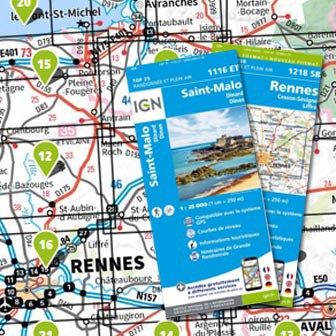
\includegraphics[width=5cm]{ressources/ign-carte.jpg}
    \captionof{figure}{L'IGN pour les particuliers}
    \label{IMG}
    \end{center}

\end{frame}
\begin{frame}
    \frametitle{Pour les professionnels}

L'IGN propose de nombreuses données et services pour créer des applications publiques, privées, militaires\dots
\end{frame}
\begin{frame}
    \frametitle{Inventaire forestier national}
    état des lieux d’une forêt en pleine évolution
    \begin{center}
    \centering
    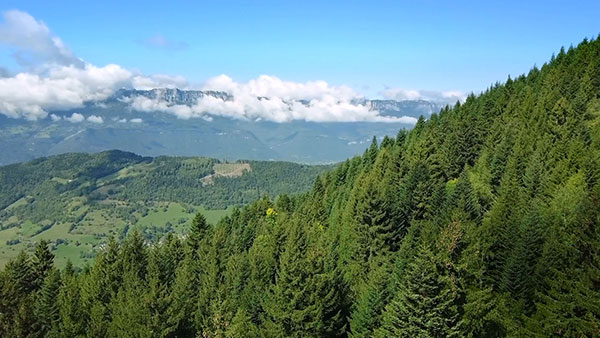
\includegraphics[width=5cm]{ressources/foret.jpg}
    \end{center}
\begin{itemize}
    \item permet de mesurer l'évolution de la mortalité des arbres.
    \item mesure le stock du bois sur pied.
\end{itemize}
\end{frame}
\begin{frame}
    \frametitle{Programme Lidar HD}
 vers une cartographie 3D du territoire 
    \begin{center}
    \centering
    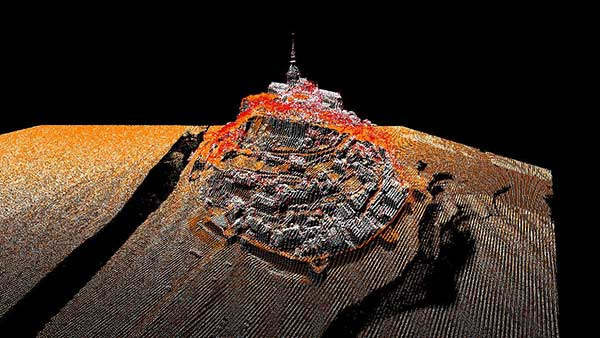
\includegraphics[width=5cm]{ressources/lidar.jpg}
    \captionof{figure}{Mont-Saint Michel}
    \label{IMG}
    \end{center}
\begin{itemize}
    \item Une précision jusqu'à 10 points par mètre carré.
\item Le projet nécessite près de 7000 heures de vol.
\item Les données produites vont représenter un volume total de 3 péta-octets (3 millions de giga-octets...)
\end{itemize}
\note[item]{GPS = précision de 5 à 10 mètres}
\note[item]{Lidar = laser imaging detection and ranging}
\end{frame}
\section{Géoportail}
\begin{frame}
    \frametitle{Géoportail}

La majorité des données sont accessibles sur le Géoportail.
\begin{center}
\centering
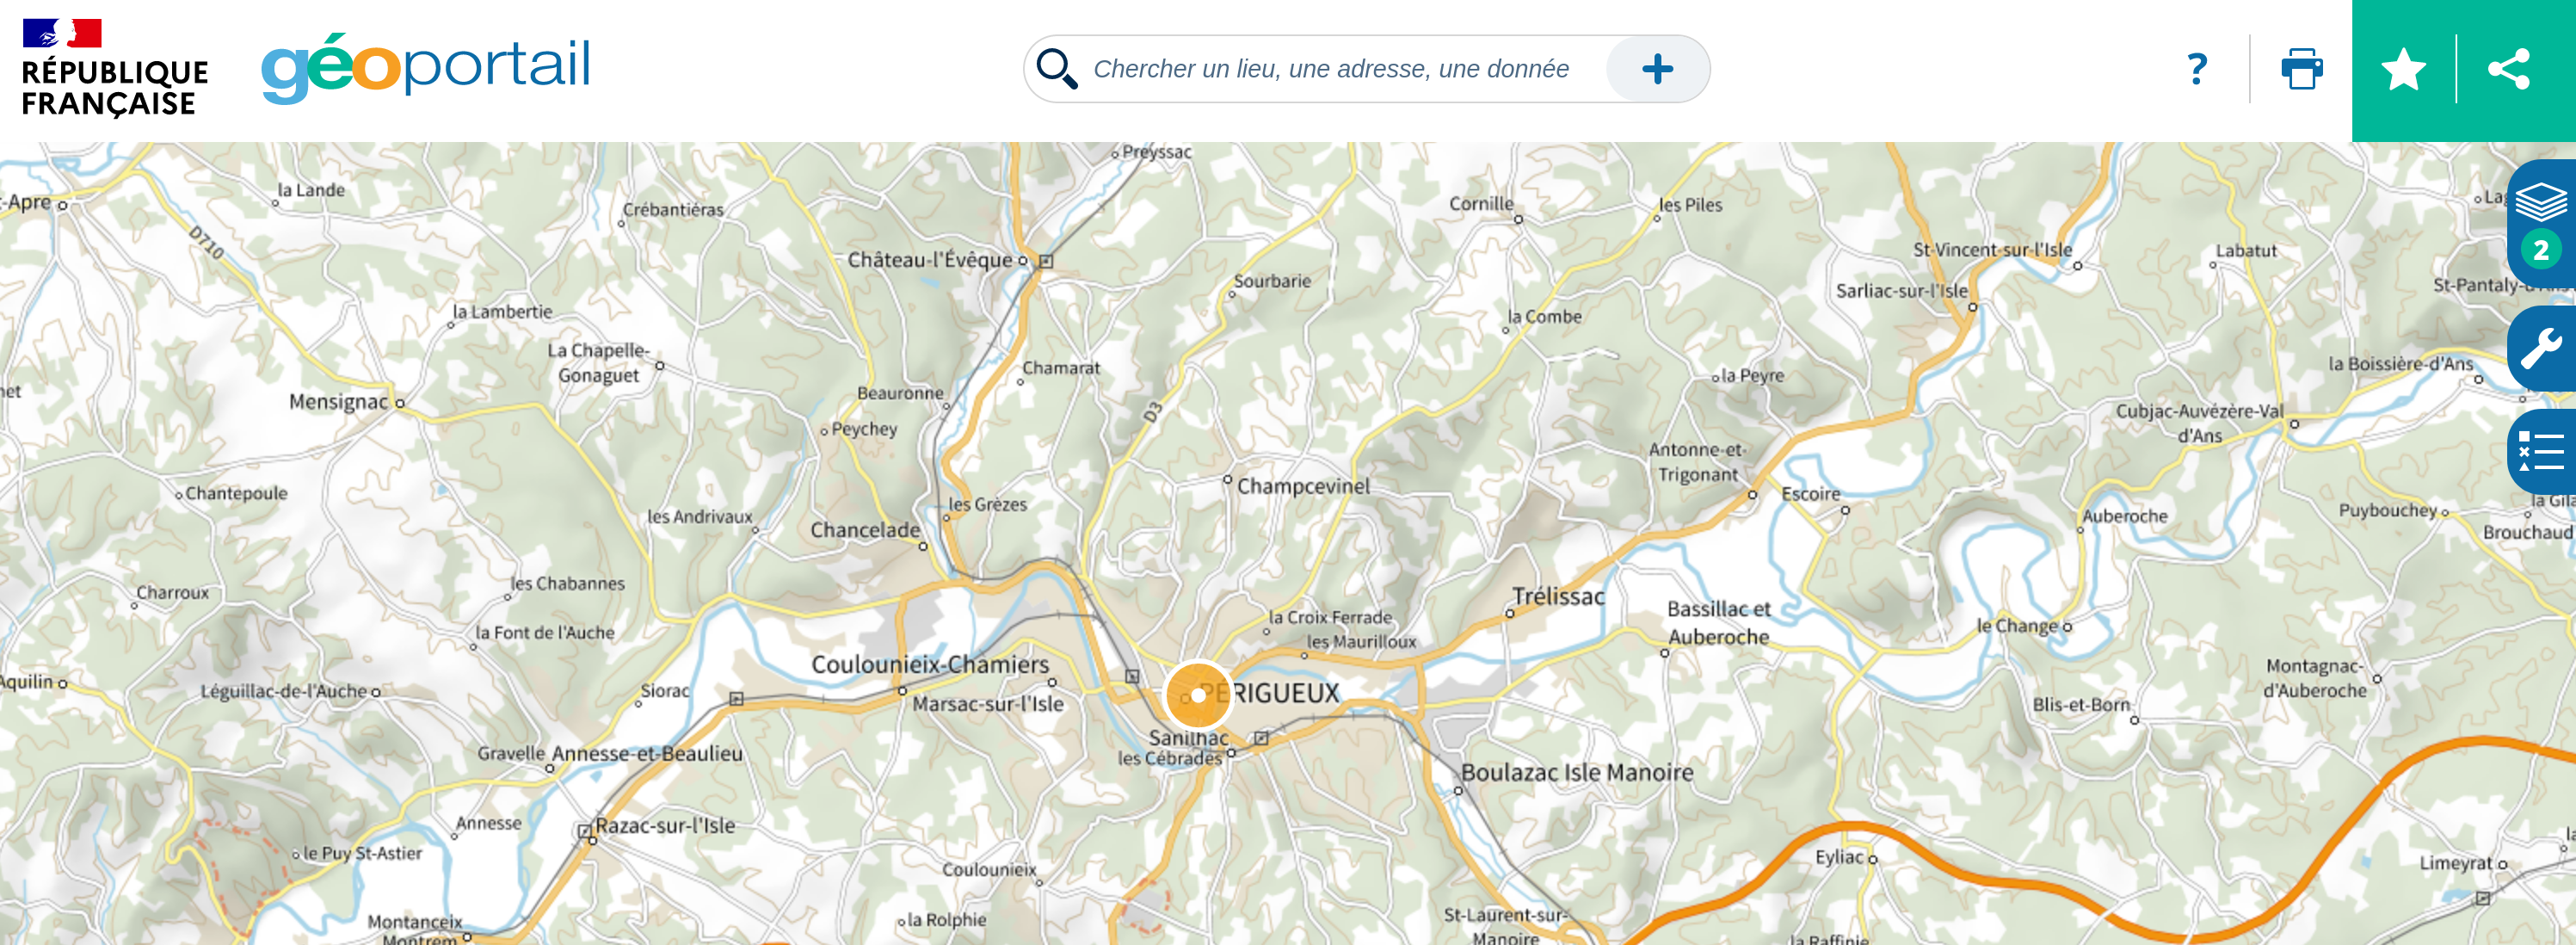
\includegraphics[width=8cm]{ressources/geoportail.png}
\captionof{figure}{Page d'accueil du Géoportail}
\label{IMG}
\end{center}
\begin{center}
    {\Large \url{https://www.geoportail.gouv.fr/}}
\end{center}
\end{frame}
\begin{frame}
    \frametitle{}

\begin{center}
\centering
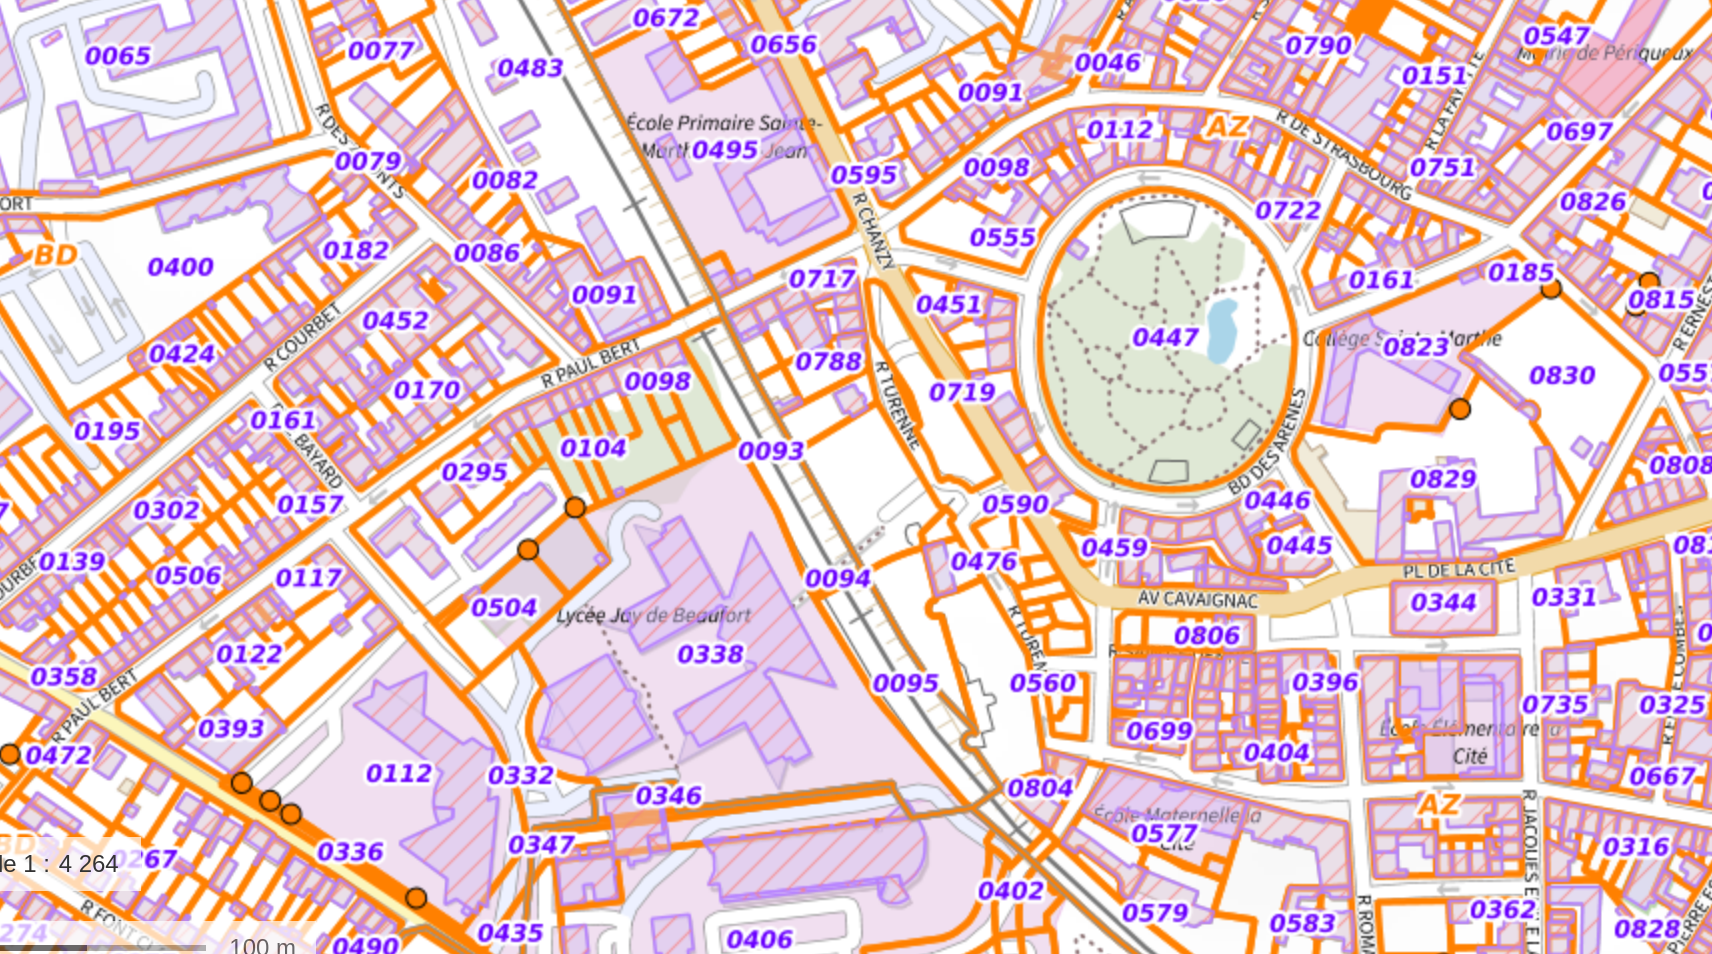
\includegraphics[width=9cm]{ressources/cadastre.png}
\captionof{figure}{Plan cadastral}
\label{IMG}
\end{center}

\end{frame}
\section{Le géocubX}
\begin{frame}
    \frametitle{Le géocubX}

    Le laboratoire d'optoélectronique, de métrologie et d’instrumentation(LOEMI) de l'IGN a développé un récepteur GPS autonome ultra-compact, ultra-précis\dots et grégaire\footnote{\url{https://www.ign.fr/publications-de-l-ign/IGNfab/Docs/Geocube-extrait-IGNMAG.pdf}}.
\begin{center}
\centering
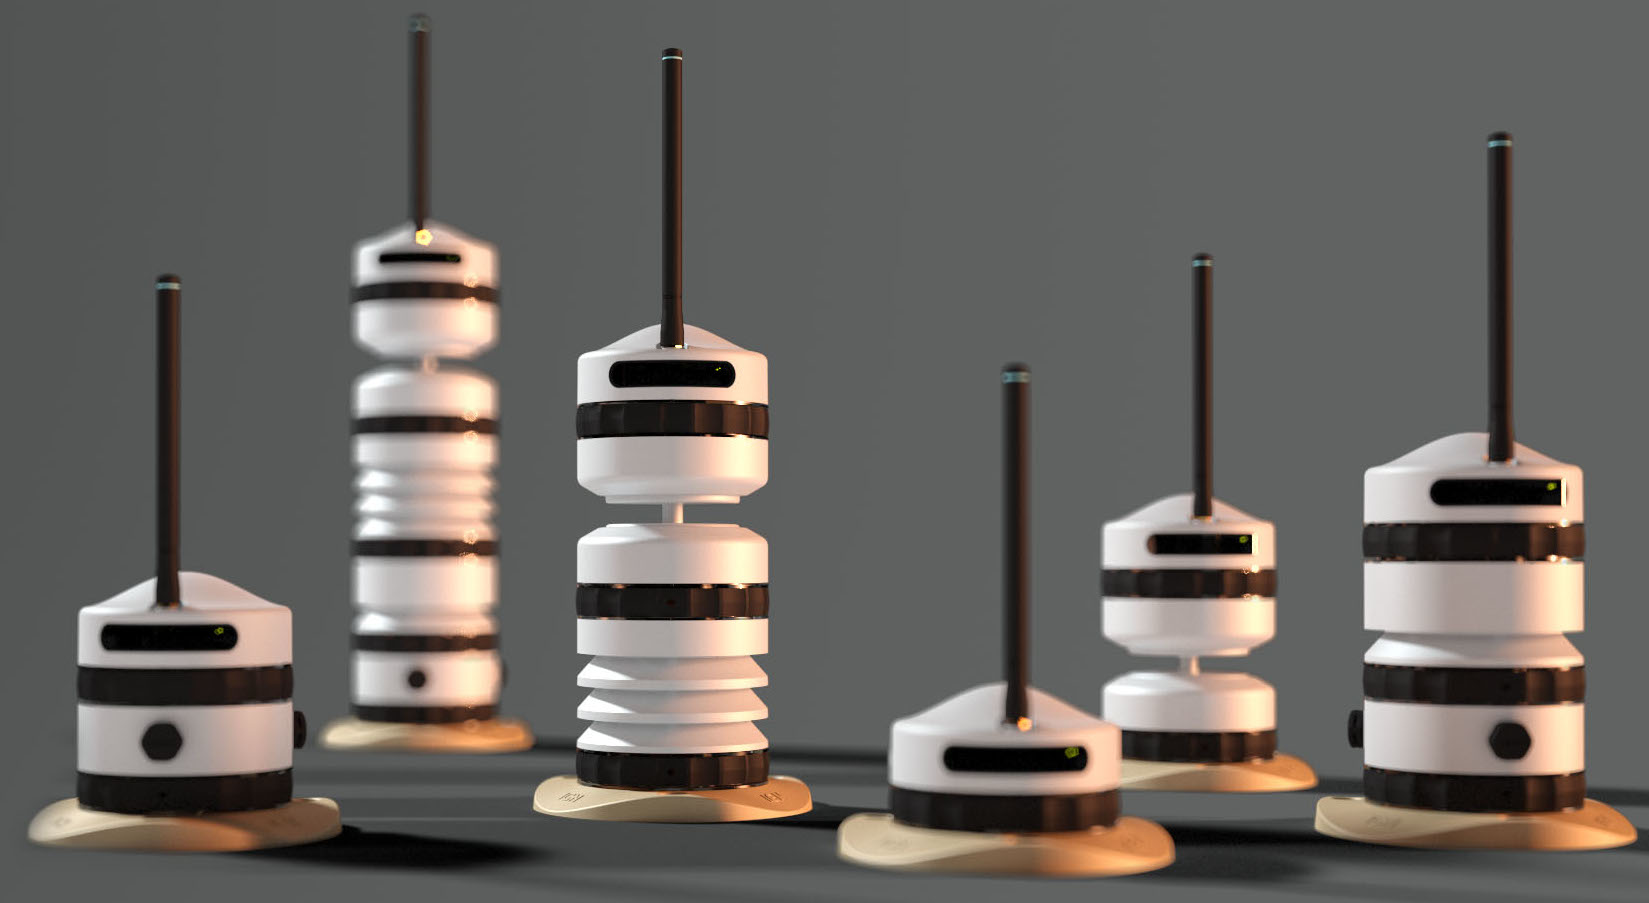
\includegraphics[width=8cm]{ressources/geocubx.jpg}
\captionof{figure}{Le géocubX, successeur du géocube.}
\end{center}

\end{frame}
\begin{frame}
    \frametitle{Supersauze}

    SuperSauze est une station de ski qui se situe sur la commune de Barcelonette. Elle subit un glissement de terrain très actif\footnote{\url{https://geocubx.com/116-2/}}.
    \begin{center}
    \centering
    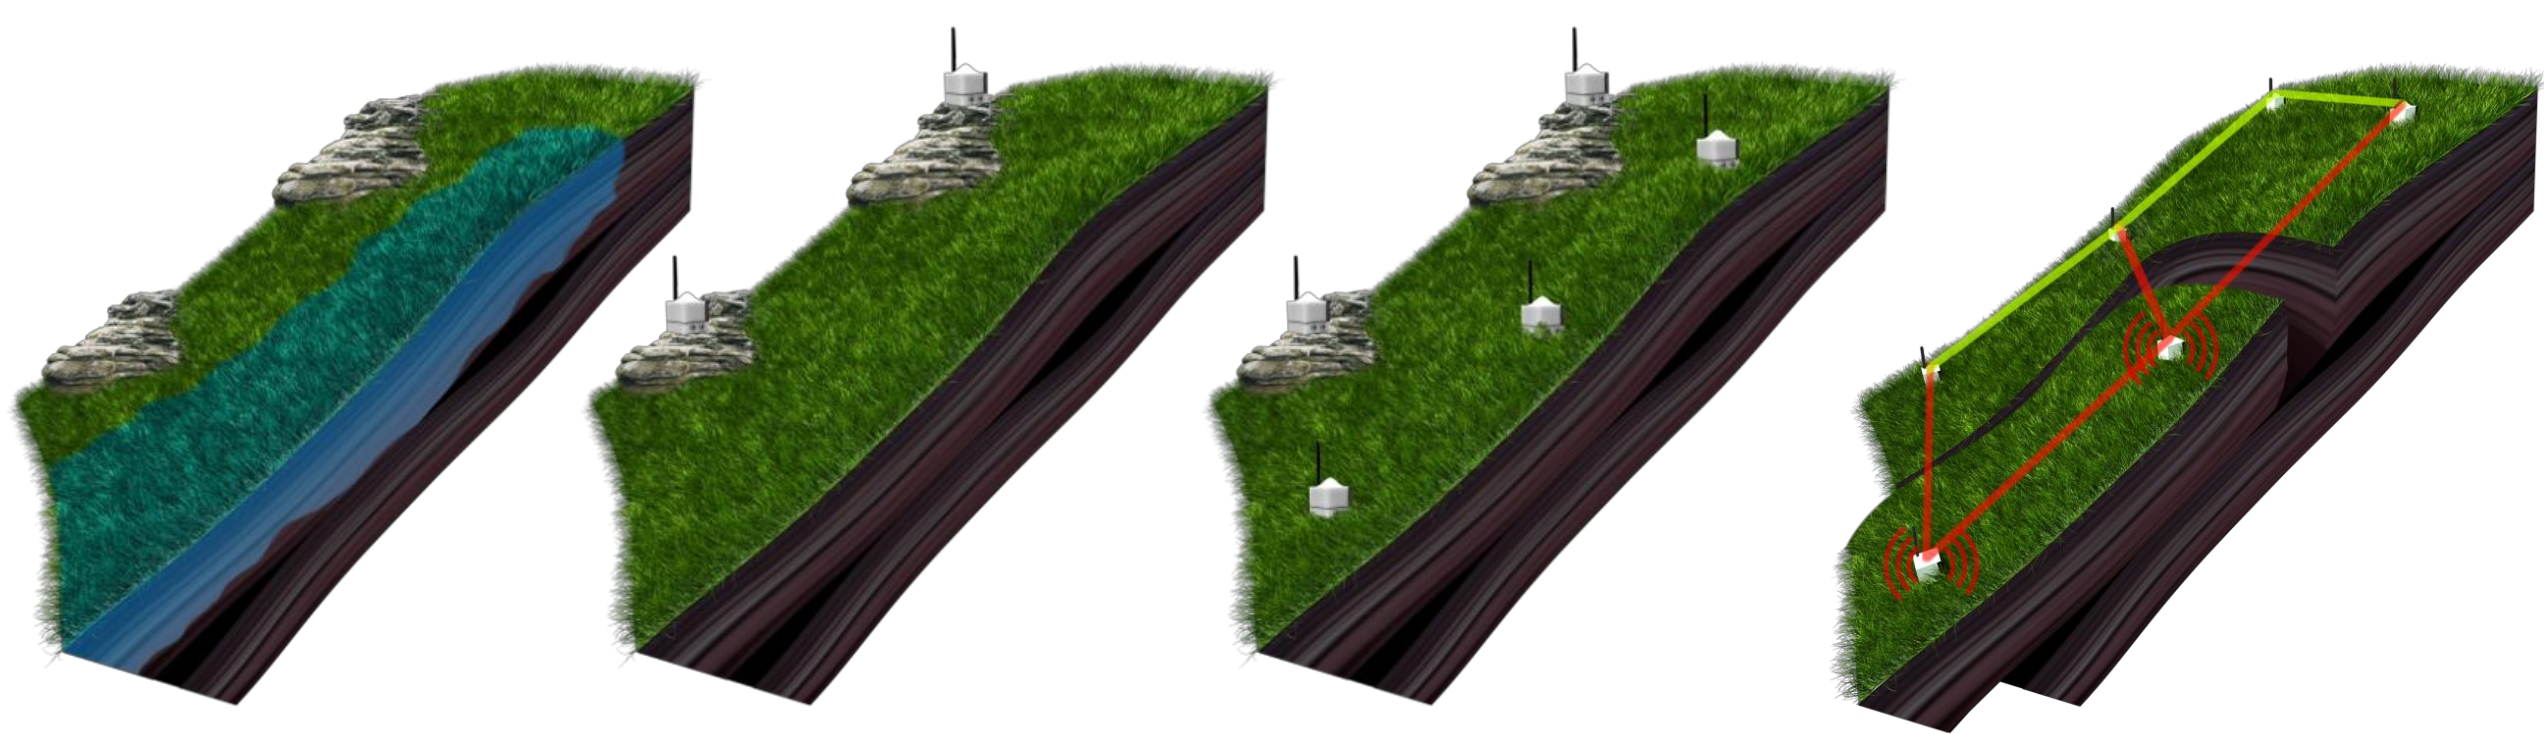
\includegraphics[width=9cm]{ressources/supersauze.png}
    \captionof{figure}{Précision obtenue en temps réel: 3mm en plani / 1cm en alti}
    \label{IMG}
    \end{center}

\end{frame}
\begin{frame}
    \frametitle{Glacier d'Argentière}

Le  glacier d’Argentière est situé au-dessus de Chamonix. Le réseau de 15 Géocubes déployé du 14 septembre au 7 novembre 2013 a permis de tester : le déploiement et le démontage rapide avec des contraintes logistiques fortes\footnote{\url{https://geocubx.com/argentiere/}}.
\begin{center}
\centering
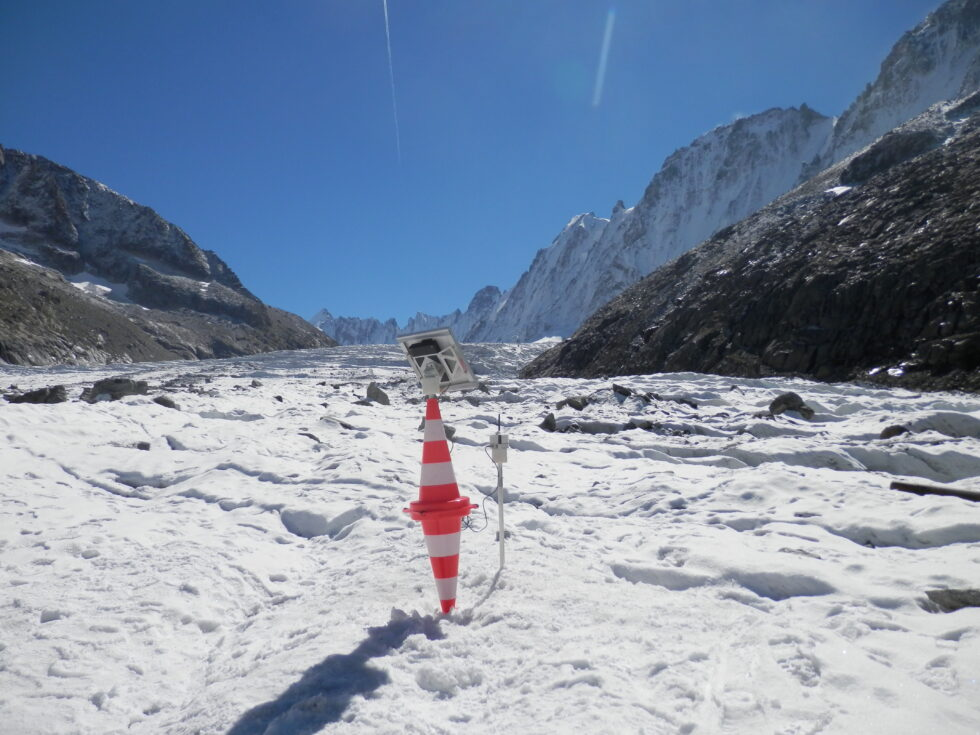
\includegraphics[width=6cm]{ressources/glacier.jpg}
\captionof{figure}{Les déplacements mesurés furent de l’ordre de 20cm/jour.}
\label{IMG}
\end{center}
\note[item]{Également surveillance Etna}
\note[item]{Antarctique}
\end{frame}
\begin{frame}
    \frametitle{Un dispositif modulaire}

    \begin{center}
    \centering
    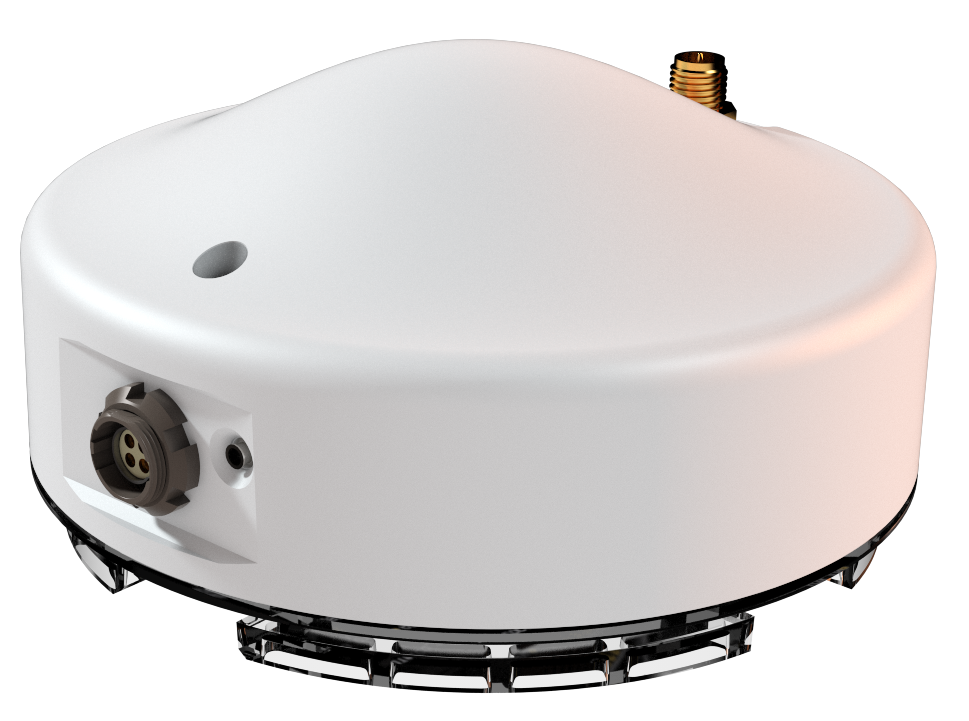
\includegraphics[width=3cm]{ressources/module.png}
    \captionof{figure}{Un module du GeocubX}
    \label{IMG}
    \end{center}
Le géocubX intègre une multitude de capteurs:
\begin{itemize}
    \item Capteur de couleur de la lumière,
    \item UVA / UVB,
    \item Anémomètre / girouette à ultrasons,
    \item Particules fines,
    \item Sonomètre,
    \item Gaz: $NO_2, O_3$,
    \item Pluviomètre,
    \item \dots
\end{itemize}
\end{frame}
\begin{frame}
    \frametitle{Un prêt de l'IGN}

\begin{center}
\centering
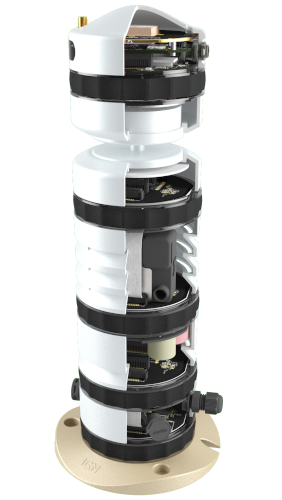
\includegraphics[width=3cm]{ressources/geocube-interne.png}
\captionof{figure}{L'IGN met à disposition un geocubX pour l'établissement.
}
\label{IMG}
\end{center}
\end{frame}
\begin{frame}
    \frametitle{Analyse des mesures}

\begin{center}
\centering
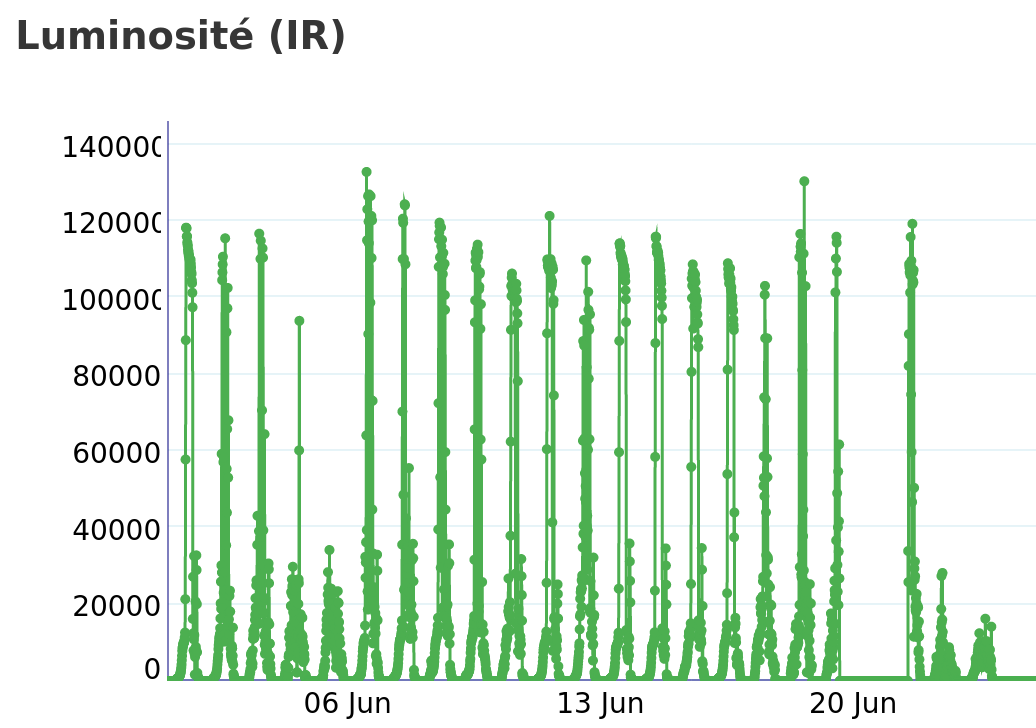
\includegraphics[width=8cm]{ressources/pression.png}
\captionof{figure}{Un site dédié pour analyser les données.}
\label{IMG}
\end{center}
\begin{center}
    {\Large \url{https://geobs.fr/cartograph/}}
\end{center}
\end{frame}
\end{document}